% Generated by make_examples.py from the model. Do not edit by hand.
\subsection{Inputs}
Table~\ref{tab:in-Challenger_3500} lists the aircraft data and the day's conditions. The example uses Wichita Dwight D. Eisenhower National (KICT) runway 01L.
\begin{table}[H]\centering\small
\begin{tabular}{@{}ll@{}}\toprule \textbf{Input} & \textbf{Value}\\\midrule
Maximum takeoff weight (MTOW) & \SI{40600}{lb} = \SI{18415.9}{kg}\\
Maximum landing weight (MLW) & \SI{34150}{lb} = \SI{15490.2}{kg}\\
Reference wing area, $S$ & \SI{48.50}{m^2} (\SI{522.0}{ft^2})\\
$C_{D_0}$ / $k$ & \num{0.030} / \num{0.045}\\
$C_{L,\max}$ takeoff / landing & \num{1.57} / \num{2.30}\\
$C_{L,\text{gnd}}$ & \num{0.30}\\
$\mu_\text{roll}$ / $\mu_\text{brake}$ & \num{0.02} / \num{0.40}\\
Sea-level static thrust, $T_\text{SLS}$ & \SI{65149}{N} (\SI{14646}{lbf})\\
Number of engines, $N_e$ & 2\\
Thrust lapse, $k_\text{lapse}$ & \num{0.90}\\
Flat rating, $\Delta T_\text{flat}$ & ISA \SI{15}{degreeCelsius}\\
Reverse thrust ratio & \num{0.30}\\
Field elevation, $h$ & \SI{1333}{ft} = \SI{406.3}{m}\\
Outside air temperature (OAT) & \SI{30}{degreeCelsius}\\
Reported wind & \ang{20} / \SI{10}{kt}\\
Runway true heading & \ang{20}\\
Runway slope (direction of travel) & \num{0.165}\,\%\\
Runway condition & Dry\\
TODA = ASDA / LDA & \SI{10302}{ft} / \SI{10302}{ft}\\
\bottomrule\end{tabular}\caption{Challenger 3500: example inputs.}\label{tab:in-Challenger_3500}\end{table}
\subsection{Step 1: Atmosphere}
Standard temperature at the field elevation, then the ISA deviation from the OAT (\eqref{eq:isa-temp} and \eqref{eq:isa-dev}):
\begin{align*}
\Theta_\text{std} &= \num{288.15} - \num{0.0065}\times\num{406.3} = \SI{285.51}{K}\\
\Delta T &= \num{30.0} - (\num{285.51} - \num{273.15}) = \SI{17.64}{degreeCelsius}\quad\text{(ISA }+17.6\text{)}
\end{align*}
Pressure, temperature, density, density ratio and speed of sound (\eqref{eq:isa-p}--\eqref{eq:isa-a}):
\begin{align*}
p &= \num{101325}\left(\frac{\num{285.51}}{\num{288.15}}\right)^{\num{5.2559}} = \SI{96538}{Pa}\\
\Theta &= \num{285.51} + \num{17.64} = \SI{303.15}{K}\\
\rho &= \frac{\num{96538}}{\num{287.05}\times\num{303.15}} = \SI{1.1094}{kg/m^3}\\
\sigma &= \frac{\num{1.1094}}{\num{1.225}} = \num{0.9056}\\
a &= \sqrt{\num{1.4}\times\num{287.05}\times\num{303.15}} = \SI{349.0}{m/s}
\end{align*}
\subsection{Step 2: Wind}
Runway components (\eqref{eq:wind-hw}--\eqref{eq:wind-xw}), then the regulatory factor \eqref{eq:wind-perf}:
\begin{align*}
V_w &= \num{10}\cos(\ang{20} - \ang{20}) = \SI{10.0}{kt}\qquad V_x = \num{10}\sin(\ang{0}) = \SI{0.0}{kt}\\
V_{w,\text{perf}} &= \num{0.5}\times\num{10.0} = \SI{5.0}{kt} = \SI{2.57}{m/s}
\end{align*}
All following steps use the performance headwind of \SI{5.0}{kt}.
\subsection{Step 3: Weight and Takeoff Speeds}
\begin{align*}
W &= m\,g_0 = \num{18415.9}\times\num{9.80665} = \SI{180598}{N}\\
V_{S1} &= \sqrt{\frac{2\times\num{180598}}{\num{1.1094}\times\num{48.50}\times\num{1.57}}} = \SI{65.39}{m/s} = \SI{127.1}{kt}\\
V_R &= \num{1.10}\,V_{S1} = \SI{71.93}{m/s} = \SI{139.8}{kt}\\
V_2 &= \num{1.20}\,V_{S1} = \SI{78.47}{m/s} = \SI{152.5}{kt}\\
V_\text{TR} &= \num{1.15}\,V_{S1} = \SI{75.20}{m/s} = \SI{146.2}{kt}
\end{align*}
\subsection{Step 4: Forces on the Ground Roll}
Thrust (\eqref{eq:jet-excess}--\eqref{eq:T-jet}). The ISA deviation of \num{17.6}\,\si{\celsius} exceeds the flat rating by \num{2.6}\,\si{\celsius}, so
\begin{gather*}
\sigma_\text{eff} = \sigma\!\left(h,\ \num{2.6}\right) = \num{0.9528}\\ T(V) = \num{65149}\times\num{0.9528}^{0.7}\left(1 - \num{0.90}\,\frac{V}{\num{349.0}}\right)
\end{gather*}
\Needspace{16\baselineskip}
Forces at brake release and at $V_R$ (\eqref{eq:eom-accel}, $C_L = C_{L,\text{gnd}} = \num{0.30}$, slope force $W\sin\theta$):
\begin{table}[H]\centering\small
\begin{tabular}{@{}lrr@{}}\toprule \textbf{Quantity} & \textbf{At $V_\text{TAS} = V_w$ (start)} & \textbf{At $V_R$}\\\midrule
Dynamic pressure $q$ (Pa) & \num{3.7} & \num{2869.8}\\
Lift $L$ (N) & \num{53} & \num{41756}\\
Drag $D$ (N) & \num{6} & \num{4739}\\
Thrust $T$ (N) & \num{62561} & \num{51298}\\
Rolling friction $\mu_\text{roll}(W-L)$ (N) & \num{3611} & \num{2777}\\
Slope force $W\sin\theta$ (N) & \num{298} & \num{298}\\
Acceleration $a$ (\si{m/s^2}) & \num{3.185} & \num{2.361}\\
\bottomrule\end{tabular}\caption{Challenger 3500: forces on the ground roll.}\end{table}
\subsection{Step 5: Ground Roll by Numerical Integration}
Equation~\eqref{eq:eom-accel} is integrated with RK45 from rest until $V_\text{TAS} = V_R$. Selected points from the solver:
\begin{table}[H]\centering\small
\begin{tabular}{@{}rrrr@{}}\toprule \textbf{$t$ (s)} & \textbf{$V_\text{TAS}$ (kt)} & \textbf{$a$ (\si{m/s^2})} & \textbf{$s$ (ft)}\\\midrule
\num{0.0} & \num{5.0} & \num{3.185} & \num{0}\\
\num{2.6} & \num{21.0} & \num{3.108} & \num{35}\\
\num{7.1} & \num{47.5} & \num{2.967} & \num{258}\\
\num{11.6} & \num{72.9} & \num{2.819} & \num{678}\\
\num{16.1} & \num{96.9} & \num{2.666} & \num{1286}\\
\num{20.6} & \num{119.5} & \num{2.511} & \num{2070}\\
\midrule \num{24.90} & \num{139.8} ($V_R$) & \num{2.361} & \num{2974}\\
\bottomrule\end{tabular}\caption{Challenger 3500: ground-roll time history (RK45 output).}\end{table}
Rotation for $t_\text{rot}$ \eqref{eq:s-rot}:
\begin{align*}
s_\text{rot} &= (\num{71.93} - \num{2.57})\times\num{3} = \SI{208.1}{m}\\
s_\text{ground} &= \num{906.5} + \num{208.1} = \SI{1114.5}{m} = \SI{3657}{ft}
\end{align*}
\subsection{Step 6: Air Distance to the Screen Height}
Climb at $V_2$ with lift equal to weight (\eqref{eq:cl-climb}--\eqref{eq:sin-gamma}); screen height \SI{35}{ft} = \SI{10.67}{m}:
\begin{align*}
q_{V_2} &= \tfrac12\times\num{1.1094}\times\num{78.47}^2 = \SI{3415.3}{Pa}, \qquad C_{L,\text{climb}} = \frac{\num{180598}}{\num{3415.3}\times\num{48.50}} = \num{1.090}\\
D &= \num{3415.3}\times\num{48.50}\times(\num{0.030} + \num{0.045}\times\num{1.090}^2) = \SI{13830}{N}, \qquad T = \SI{50237}{N}\\
\sin\gamma &= \frac{\num{50237} - \num{13830}}{\num{180598}} = \num{0.2016}, \qquad \gamma = \SI{0.2030}{rad}, \qquad \text{gradient} = \num{20.6}\,\%
\end{align*}
Transition arc (\eqref{eq:R-tr}--\eqref{eq:h-tr}):
\begin{align*}
R_\text{TR} &= \frac{\num{75.20}^2}{\num{9.807}\times(\num{1.2} - 1)} = \SI{2883.1}{m}\\
h_\text{TR} &= \num{2883.1}\,(1 - \cos \num{0.2030}) = \SI{59.19}{m}
\end{align*}
Since $h_\text{TR} \ge h_\text{scr}$, the screen is cleared inside the arc \eqref{eq:s-air-arc}:
\begin{equation*}
s_\text{air} = \sqrt{\num{2883.1}^2 - (\num{2883.1} - \num{10.67})^2} = \SI{247.8}{m}
\end{equation*}
Corrected for wind \eqref{eq:s-air-wind}, then the takeoff distance \eqref{eq:tod}:
\begin{align*}
s_\text{air} &= \num{247.8}\times\frac{\num{75.20} - \num{2.57}}{\num{75.20}} = \SI{239.3}{m}\\
\text{TOD}_\text{AEO} &= \num{1114.5} + \num{239.3} = \SI{1353.8}{m} = \SI{4442}{ft}
\end{align*}
\subsection{Step 7: Balanced Field Length}
For each trial $V_1$, the accelerate-go and accelerate-stop distances are computed (\eqref{eq:s-go}--\eqref{eq:s-stop}) and their difference $f(V_1)$ \eqref{eq:f-v1}:
\begin{table}[H]\centering\small
\begin{tabular}{@{}rrrr@{}}\toprule \textbf{$V_1$ (kt)} & \textbf{$s_\text{go}$ (ft)} & \textbf{$s_\text{stop}$ (ft)} & \textbf{$f(V_1)$ (ft)}\\\midrule
\num{69.9} & \num{7586} & \num{1298} & \num{6288}\\
\num{87.4} & \num{7094} & \num{2038} & \num{5056}\\
\num{104.9} & \num{6438} & \num{2957} & \num{3481}\\
\num{118.8} & \num{5772} & \num{3828} & \num{1945}\\
\num{129.3} & \num{5176} & \num{4564} & \num{612}\\
\num{139.8} & \num{4482} & \num{5375} & \num{-893}\\
\midrule \textbf{\num{133.7}} & \textbf{\num{4896}} & \textbf{\num{4896}} & \textbf{\num{-0.0}}\\
\bottomrule\end{tabular}\caption{Challenger 3500: accelerate-go and accelerate-stop against trial $V_1$.}\end{table}
$f$ changes sign between the trial values, so Brent's method converges to the balanced $V_1 = \SI{133.7}{kt}$ (bold row). Then (\eqref{eq:bfl}--\eqref{eq:tofl}):
\begin{align*}
\text{BFL} &= \SI{4896}{ft}\\
1.15\times\text{TOD}_\text{AEO} &= 1.15\times\num{4442} = \SI{5108}{ft}\\
\text{TOFL} &= \max\left(\num{4896},\ \num{5108}\right) = \SI{5108}{ft} = \SI{1557}{m}
\end{align*}
The TOFL is set by the all-engines distance with its 15\% margin. The one-engine-inoperative climb gradient at $V_2$ is \num{6.3}\,\%.
\begin{figure}[H]\centering
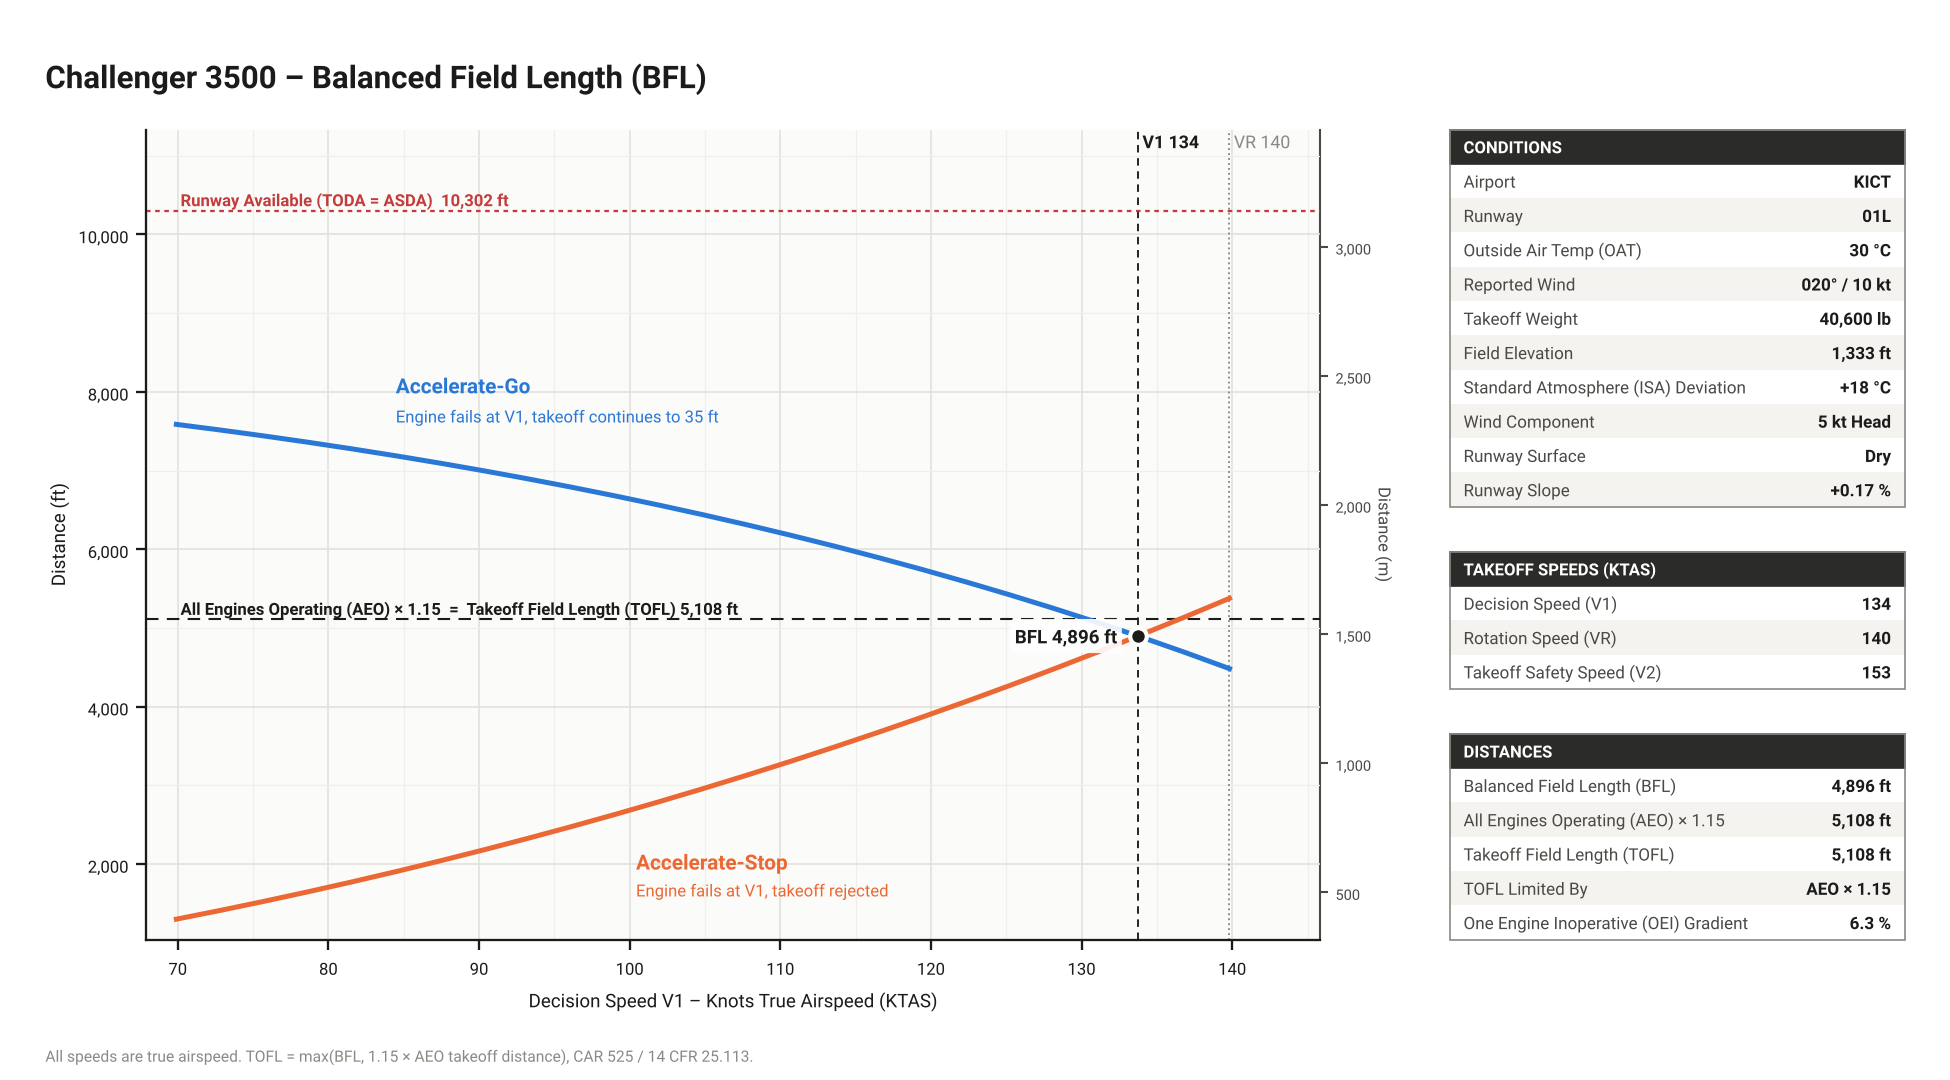
\includegraphics[width=\linewidth]{figures/bfl_example_Challenger_3500.png}
\caption{Challenger 3500: Balanced Field Length (BFL) for this example.}\end{figure}
\subsection{Step 8: Landing}
Landing at MLW on the same runway, no reverse thrust credit (\eqref{eq:vref}--\eqref{eq:ldr}):
\begin{align*}
V_{S0} &= \sqrt{\frac{2\times\num{151907}}{\num{1.1094}\times\num{48.50}\times\num{2.30}}} = \SI{49.55}{m/s} = \SI{96.3}{kt}\\
V_\text{REF} &= \num{1.30}\,V_{S0} = \SI{125.2}{kt}, \qquad V_\text{TD} = \num{1.15}\,V_{S0} = \SI{110.8}{kt}\\
s_\text{air} &= \frac{\num{15.24}}{\tan\ang{3}}\times\frac{\num{64.41} - \num{2.57}}{\num{64.41}} = \SI{279.2}{m}\\
s_\text{free} &= (\num{56.98} - \num{2.57})\times\num{3} = \SI{163.2}{m}\\
s_\text{brake} &= \SI{367.7}{m} \quad\text{(\eqref{eq:eom-brake} integrated to rest, \num{13.6}\,s)}\\
\text{LD} &= \num{279.2} + \num{163.2} + \num{367.7} = \SI{810.1}{m} = \SI{2658}{ft}
\\ \text{LDR} &= \frac{\num{810.1}}{0.6} = \SI{1350.2}{m} = \SI{4430}{ft}
\end{align*}
\subsection{Step 9: Runway Check}
\begin{table}[H]\centering\small
\begin{tabular}{@{}lrlrrl@{}}\toprule \textbf{Required} & \textbf{ft} & \textbf{Available} & \textbf{ft} & \textbf{Margin (ft)} & \textbf{Result}\\\midrule
Takeoff Field Length (TOFL) & \num{5108} & TODA & \num{10302} & \num{5194} & OK\\
Accelerate-Stop Distance (ASD) & \num{4896} & ASDA & \num{10302} & \num{5406} & OK\\
Landing Distance Required (LDR) & \num{4430} & LDA & \num{10302} & \num{5872} & OK\\
\bottomrule\end{tabular}\caption{Challenger 3500: runway check, KICT runway 01L.}\end{table}
